\documentclass[12pt, letterpaper]{article}
\usepackage{graphicx}
\usepackage[T1]{fontenc}
\usepackage[polish]{babel}
\usepackage[utf8]{inputenc}
\usepackage{times}


\graphicspath{{images/}}

%--------------------------------------------------------------------------------------------------
%       TITLE SECTION
%--------------------------------------------------------------------------------------------------
\begin{titlepage}

\begin{center}
	
\includegraphics[scale=0.2]{ur_inf_logo}\\ \\ \\ \\
\end{center}

\begin{center}

	{ \huge \bfseries Inżynieria oprogramowania}\\[0.4cm] 

	\textsc{\Large PandaVision}\\[0.5cm] \\ \\ \\ \\ 
	
	\vspace{0.8cm}	
	
	\emph{Autor:} \\
	\textbf{Oskar Paśko} (117987)\\
	
	
	\vspace{0.8cm}
	
	\emph{Kierunek:} \\
	Informatyka i ekonometria
	
	\vspace{8cm}
	
	\emph{Prowadzący:} \\
	mgr inż. Ewa Żesławska\\ \\ \\ \\ 
	
	\vspace{2cm}
	
	Rzeszów, 2023
\end{center}
\end{titlepage}

\usepackage{geometry}
 \geometry{
 a4paper,
 total={170mm,257mm},
 left=25mm,
 top=25mm,
 right=25mm,
 bottom=25mm 
 }
 
%--------------------------------------------------------------------------------------------------
%       BEGIN DOCUMENT
%--------------------------------------------------------------------------------------------------

\begin{document}
\newpage

%--------------------------------------------------------------------------------------------------
%       TABLE OF CONTENTS
%--------------------------------------------------------------------------------------------------
\tableofcontents

\newpage

%--------------------------------------------------------------------------------------------------
%       OPIS ŚWIATA RZECZYWISTEGO
%--------------------------------------------------------------------------------------------------

\section{Opis świata rzeczywistego}

	\subsection{Opis zasobów ludzkich}

	Gra na urządzenia wirtualnej rzeczywistości takich jak Oculus Quest 2 polegająca na zabawie kolorami z użyciem sześcianów lub innych obiektów na różnych planszach. Gra ma pomagać nad diagnozowaniem ewentualnych schorzeń daltonizmu lub jemu podobnych. Aplikacja może być również używana do zabawy rywalizacyjnej. Gra powinna być przystosowana dla użytkownika w dowolnym wieku. Gra pozwala na zapisywanie za pomocą eye-trackera ścieżki wzroku z jaką badany podążał podczas rozgrywki. Podczas rozgrywki mierzymy również czas wykonania zadania. Dzięki wynikom czasu, poprawności oraz ścieżkom eye-trackera jesteśmy w stanie bardzo dobrze przeanalizować zachowanie gracza oraz stwierdzić podejrzenie schorzenia. Wszystkie wyniki oraz przebieg badań jest zapisywany w postaci danych w bazie danych, do której dostęp ma administrator.
	

	\subsection{Przepisy i strategia firmy}
	
	Strategią firmy jest pomoc dzieciom oraz osobom dorosłym w diagnozowaniu schorzeń takich jak daltonizm itp. Dążymy do jak najlepszego kontaktu z naszymi użytkownikami. Chcemy żeby nasi użytkownicy mieli jak największy wpływ na rozwój oprogramowania, które jest tworzone bezpośrednio dla nich. Przewidywane są częste aktualizacje oprogramowania w celu poprawy działania aplikacji oraz dodawanie nowych funkcjonalności i badań w przyszłości. Aplikacja dodatkowo będzie wysyłać w przeciągu tygodnia wyniki z najnowszych badań razem z ich interpretacją i ewentualnymi zaleceniami. Dodatkowo priorytetem firmy będzie zadbanie o bezpieczeństwo wrażliwych danych osobowych oraz danych konta naszych użytkowników.
	

	\subsection{Dane techniczne}
	
	Użytkownicy mogą korzystać z aplikacji tylko na urządzeniach wirtualnej rzeczywistości. Użytkownicy mogą się zalogować do aplikacji tylko wtedy gdy mają połączenie z internetem. Jeśli użytkownik nie posiada konta może je darmowo utworzyć. Zarejestrowany użytkownik może się zalogować za pomocą unikatowego numeru telefonu oraz hasła. Aplikacja umożliwia kontakt z administratorem w celu weryfikacji oraz konsultacji przeprowadzonych badań.
	
%--------------------------------------------------------------------------------------------------
%       WYMAGANIA FUNKCJONALNE I NIEFUNKCJONALNE
%--------------------------------------------------------------------------------------------------

	\subsection{Wymagania funkcjonalne i niefunkcjonalne}

		\subsubsection{Wymagania funkcjonalne}
		
			\begin{itemize}
				\item Logowanie do systemu za pomocą adresu email i hasła
				\item Możliwość zarejestrowania się do systemu
				\item Możliwość przeglądania historii badań
				\item Możliwość przeczytania opisów poszczególnych badań,
				\item Możliwość wyboru badań z listy,
				\item Wykonanie badania wybranego z listy,
			\end{itemize}
			
		\subsubsection{Wymagania niefunkcjonalne}
		
			\begin{itemize}
				\item Aplikacja zapewnia bezpieczeństwo wrażliwych danych,
				\item Aplikacja jest prosta w obsłudze,
				\item Aplikacja zapewnia schludny i przejrzysty interface,
				\item Aplikacja działa na urządzeniach wirtualnych Oculus Quest 2,
				\item Aplikacja jest tworzona w środowisku Unity,
				\item Aplikacja wykorzystuje bazę danych
			\end{itemize}
			
%--------------------------------------------------------------------------------------------------
%      	REQUREMENT DIAGRAM
%--------------------------------------------------------------------------------------------------
			
		\subsection{Requirement Diagram}
		
		W oparciu o opis świata rzeczywistego oraz zdefiniowane wymagania funkcjonalne i funkcjonalne na Rys.1 przedstawiono diagram wymagań dla opisywanego oprogramowania.
		
		\begin{center}
			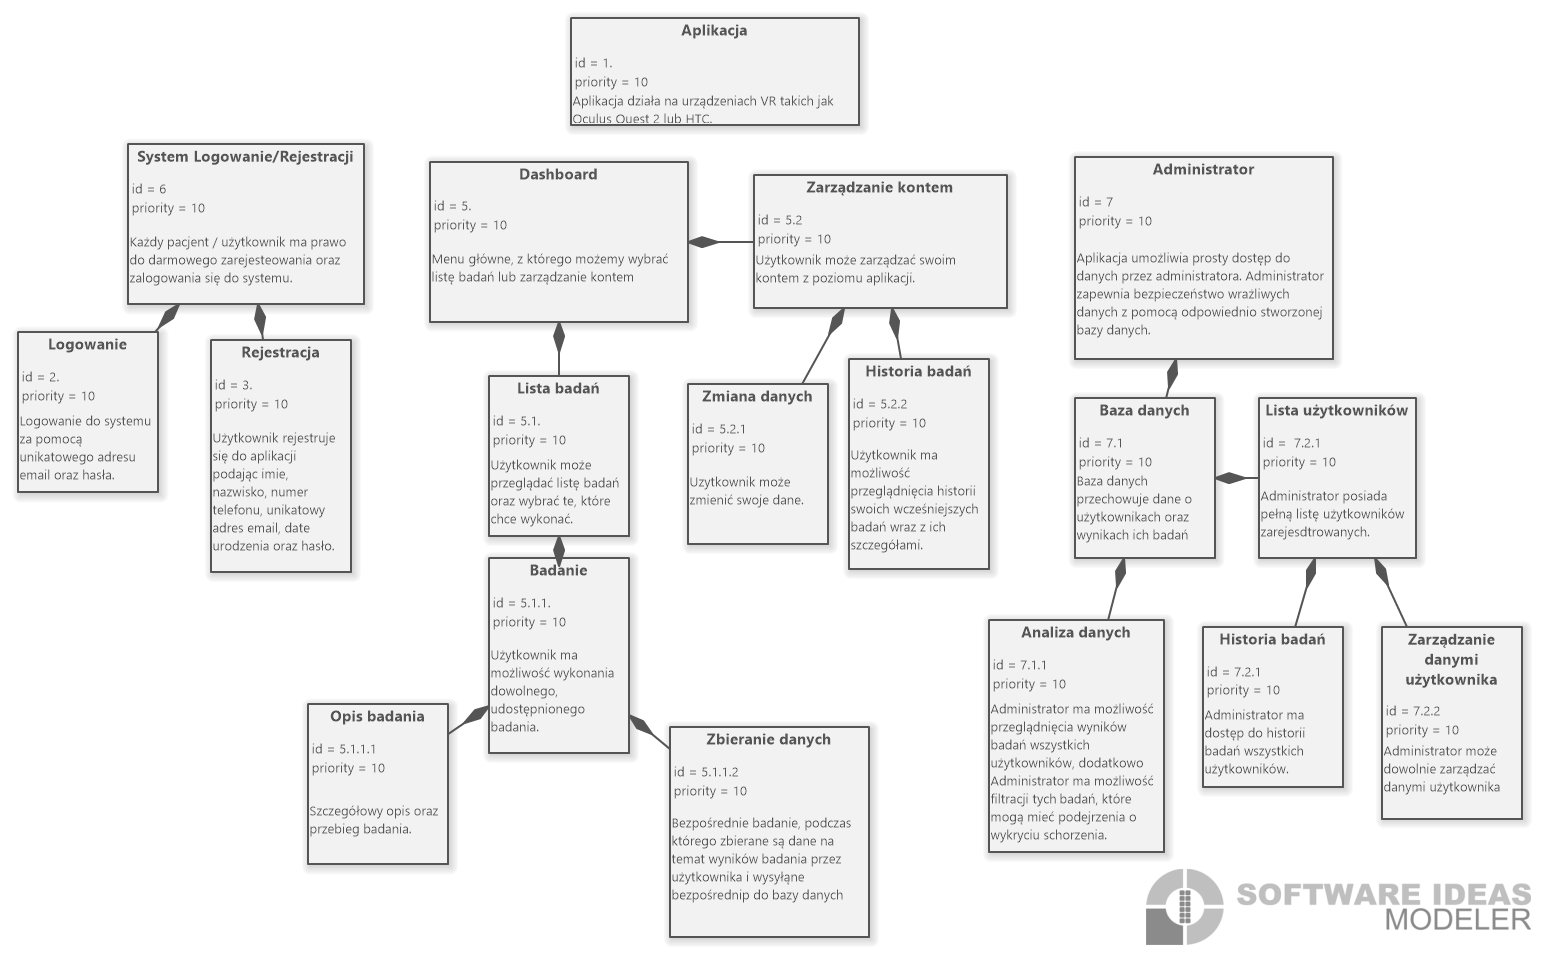
\includegraphics[scale=0.4]{reqDiagram}\\
			\caption{Rys.1 Diagram wymagań}
		\end{center}
		
%--------------------------------------------------------------------------------------------------
%       DIAGRAMY UML
%--------------------------------------------------------------------------------------------------
		
		\section{Diagramy UML}
		\subsection{Diagram przypadków użycia}
		
		\begin{center}
			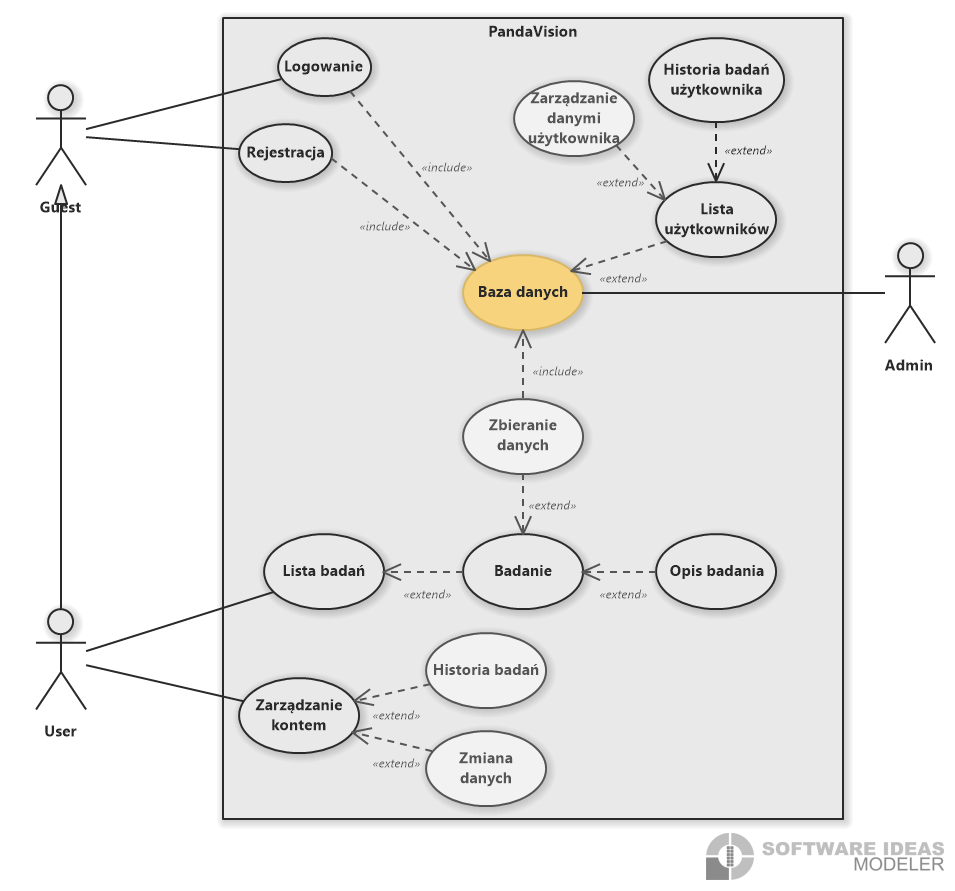
\includegraphics[scale=0.5]{useCaseDiagram}\\
			\caption{Rys.2 Diagram przypadków użycia}
		\end{center}		
		
		\textbf{Definicje scenariuszy przypadków użycia} (PU - przypadek użycia, WS - warunki wstępne, WK - warunki końcowe)\\
		
		\newpage
		
%--------------------------------------------------------------------------------------------------
%       DEFINICJA AKTORÓW
%--------------------------------------------------------------------------------------------------
		
		\subsubsection{Definicja aktorów}
		
		\quad		
		
		\textbf{Aktor:} Gość\\
		
		\textbf{Opis:} Gość może się zalogować lub zarejestrować do systemu.\\
		
		\textbf{Przypadki użycia:}
		
		\begin{itemize}
			\item PU Logowanie
			\item PU Rejestracja
		\end{itemize}
		
		\vspace{1cm}
		
		\textbf{Aktor:} Użytkownik\\
		
		\textbf{Opis:} Użytkownik oprócz funkcjonalności gości może przeglądać listę badań, opisy badań oraz historie swoich badań. Użytkownik może również zacząć dowolne badanie dostępne z listy.\\
		
		\textbf{Przypadki użycia:}
		
		\begin{itemize}
			\item PU Opis badań
			\item PU Historia badań
			\item PU Lista badań powiązane przez << extend >> z PU Opis badania oraz powiązane przez\\ << extend >> z PU Badanie
		\end{itemize}
		
		\vspace{1cm}
		
		\textbf{Aktor:} Administrator\\
		
		\textbf{Opis:} Administrator zarządza systemem, bazą danych oraz analizuje wyniki badań użytkowników.\\
		
		\textbf{Przypadki użycia:}
		
		\begin{itemize}
			\item PU Lista użytkowników powiązane przez << extend >> z PU Historia badań użytkownika
		\end{itemize}		
		
		\newpage
		
%-------------------------------------------
%       PU Baza danych
%-------------------------------------------	
		
		\subsubsection{PU Baza danych}
		
		\quad
		
		\textbf{Cel: }\\
		
		WS: \\
		
		WK: \\
		
		\textbf{Przebieg:}\\
		 \\
		
		
%-------------------------------------------
%       PU LOGOWANIE
%-------------------------------------------	
		
		\subsubsection{PU Logowanie}
		
		\quad
		
		\textbf{Cel: Zalogowanie do systemu}\\
		
		WS: może być wywołany z PU Logowanie\\
		
		WK: podanie niezbędnych danych do zalogowania tj. adres e-mail i hasło\\
		
		\textbf{Przebieg:}\\
		Logowanie dostępne jest poprzez zakładkę "Logowanie". Podczas logowania należy podać adres e-mail oraz hasło. W przypadku podania błędnych danych pojawi się informacja o niepowodzeniu logowania w postaci komunikatu "Podano błędne dane". Użytkownik może ponownie podać dane lub wyjść z aplikacji. W przypadku 5 błędnych logowań system zablokuje konto i wyświetli komunikat "Prosimy o kontakt w celu odblokowania konta". Jeśli użytkownik wprowadzi poprawne dane to użytkownik zostanie zalogowany do systemu i przeniesie się automatycznie do panelu głównego aplikacji.\\
		
%-------------------------------------------
%       PU REJESTRACJA
%-------------------------------------------	
		
		\subsubsection{PU Rejestracja}
		
		\quad
		
		\textbf{Cel: Rejestracja do systemu}\\
		
		WS: może być wywołany z PU Rejestracja\\
		
		WK: podanie niezbędnych danych do zalogowania tj. imię, nazwisko, adres e-mail, hasło, numer telefonu, data urodzenia\\
		
		\textbf{Przebieg:}\\
		Rejestracja jest dostępna przez zakładkę "Rejestracja". Podczas rejestracji należy podać imię, nazwisko, datę urodzenia, numer telefonu, unikalny adres e-mail oraz hasło. W przypadku podania niewłaściwych danych np. numeru telefonu o długości 10 cyfr lub adresu e-mail bez znaku "@" wyskoczy komunikat "Wprowadzono nieprawidłowe dane". W przypadku podania adresu e-mail, który już jest przypisany do innego konta wyskoczy komunikat "Konto z podanym adresem e-mail już istnieje". Użytkownik może ponownie podać dane lub wyjść z aplikacji. Jeśli użytkownik wprowadzi poprawne dane to zostanie przekierowany do panelu logowania, gdzie będzie mógł się zalogować odpowiednimi danymi. \\
		
%-------------------------------------------
%       PU LISTA BADAŃ
%-------------------------------------------	
		
		\subsubsection{PU Lista badań}
		
		\quad
		
		\textbf{Cel: Wybór badania z listy}\\
		
		WS: może być wywołany z PU Lista badań\\
		
		WK: wybór oraz wykonanie badania z listy\\
		
		\textbf{Przebieg:}\\
		Lista badań jest dostępna przez zakładkę "Lista badań". Użytkownik może przeglądać dostępne badania, które są zaprezentowane w postaci listy za pomocą nazw badań oraz miniaturki zrzutu ekranu z przebiegu badania. Po kliknięciu w wybrane badanie użytkownik zostanie przekierowany do panelu badania. W panelu będzie mógł przeczytać szczegółowy opis badania przez wybranie zakładki "Opis badania", kryteria jakie będą brane pod uwagę, czas trwania badania oraz zacząć badanie. \\
		
%-------------------------------------------
%       PU Badanie
%-------------------------------------------	
		
		\subsubsection{PU Badanie}
		
		\quad
		
		\textbf{Cel: }\\
		
		WS: \\
		
		WK: \\
		
		\textbf{Przebieg:}\\
		 \\
		 
%-------------------------------------------
%       PU Opis Badania
%-------------------------------------------	
		
		\subsubsection{PU Opis Badania}
		
		\quad
		
		\textbf{Cel: }\\
		
		WS: \\
		
		WK: \\
		
		\textbf{Przebieg:}\\
		 \\
		 
%-------------------------------------------
%       PU Zarządzanie kontem
%-------------------------------------------	
		
		\subsubsection{PU Zarządzanie kontem}
		
		\quad
		
		\textbf{Cel: }\\
		
		WS: \\
		
		WK: \\
		
		\textbf{Przebieg:}\\
		 \\
		 
%-------------------------------------------
%       PU Historia badań
%-------------------------------------------	
		
		\subsubsection{PU Historia badań}
		
		\quad
		
		\textbf{Cel: }\\
		
		WS: \\
		
		WK: \\
		
		\textbf{Przebieg:}\\
		 \\
		 
%-------------------------------------------
%       PU Zmiana danych
%-------------------------------------------	
		
		\subsubsection{PU Zmiana danych}
		
		\quad
		
		\textbf{Cel: }\\
		
		WS: \\
		
		WK: \\
		
		\textbf{Przebieg:}\\
		 \\
			
		
%-------------------------------------------
%       PU LISTA UŻYTKOWNIKÓW
%-------------------------------------------	
		
		\subsubsection{PU Lista użytkowników}
		
		\quad
		
		\textbf{Cel: Przeglądanie listy użytkowników}\\
		
		WS: może być wywołany z PU Lista użytkowników\\
		
		WK: Przeglądanie danych użytkowników \\
		
		\textbf{Przebieg:}\\
		Jeśli administrator prawidłowo zaloguje się do systemu to zostaje wyświetlona w panelu głównym lista użytkowników zarejestrowanych do systemu w postaci listy. Lista jest reprezentowana za pomocą imienia, nazwiska oraz adresu e-mail użytkownika. Klikając w użytkownika z listy możemy przejść do szczegółów jego konta.\\	
		
%-------------------------------------------
%       PU HISTORIA BADAŃ UŻYTKOWNIKA
%-------------------------------------------	
		
		\subsubsection{PU Historia badań użytkownika}
		
		\quad
		
		\textbf{Cel: Przeglądanie historii badań użytkownika}\\
		
		WS: może być wywołany z PU Historia badań użytkownika\\
		
		WK: Przeglądanie historii badań użytkownika \\
		
		\textbf{Przebieg:}\\
		Po wybraniu użytkownika z list administrator zobaczy listę badań konkretnego użytkownika. Wyświetlane będą takie informacje jak: data badania, rodzaj badania oraz wyniki badań, dodatkowo powinny być pokazane pliki do pobrania, które stworzyły się podczas badania jak np. ścieżka śledzenia wzroku lub wykresy danych dostarczonych podczas badania. W przypadku stwierdzenia podejrzenia choroby poprzez nieprawidłowości związane z badaniem administrator przez zakładkę "Kontakt" powinien mieć bezpośrednią możliwość wysłania na adres e-mail użytkownika informacji na temat wyników badania wraz z udostępnieniem wszelkich danych oraz plików.
		
%-------------------------------------------
%       PU Zarządzanie danymi użytkownika
%-------------------------------------------	
		
		\subsubsection{PU Zarządzanie danymi użytkownika}
		
		\quad
		
		\textbf{Cel: }\\
		
		WS: \\
		
		WK: \\
		
		\textbf{Przebieg:}\\
		 \\
		

		

%--------------------------------------------------------------------------------------------------
%       DIAGRAM AKTYWNOŚCI
%--------------------------------------------------------------------------------------------------
		\subsection{Diagram aktywności}
		
		\subsubsection{Diagram aktywności - Logowanie}
		
		\begin{center}
			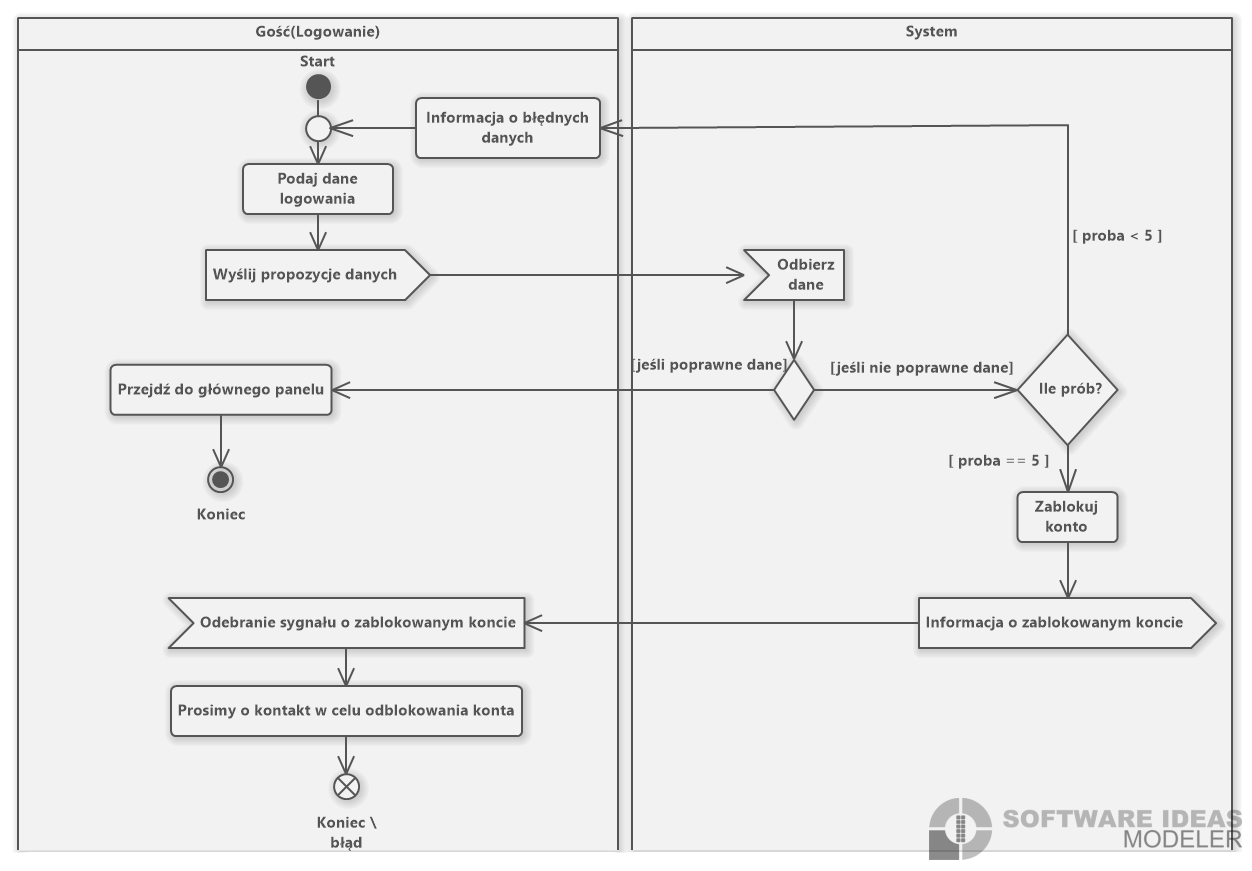
\includegraphics[scale=0.5]{aclogowanie}\\
			\caption{Rys.3 Diagram aktywności - Logowanie}
		\end{center}	
		
		\subsubsection{Diagram aktywności - Rejestracja}
		
		\begin{center}
			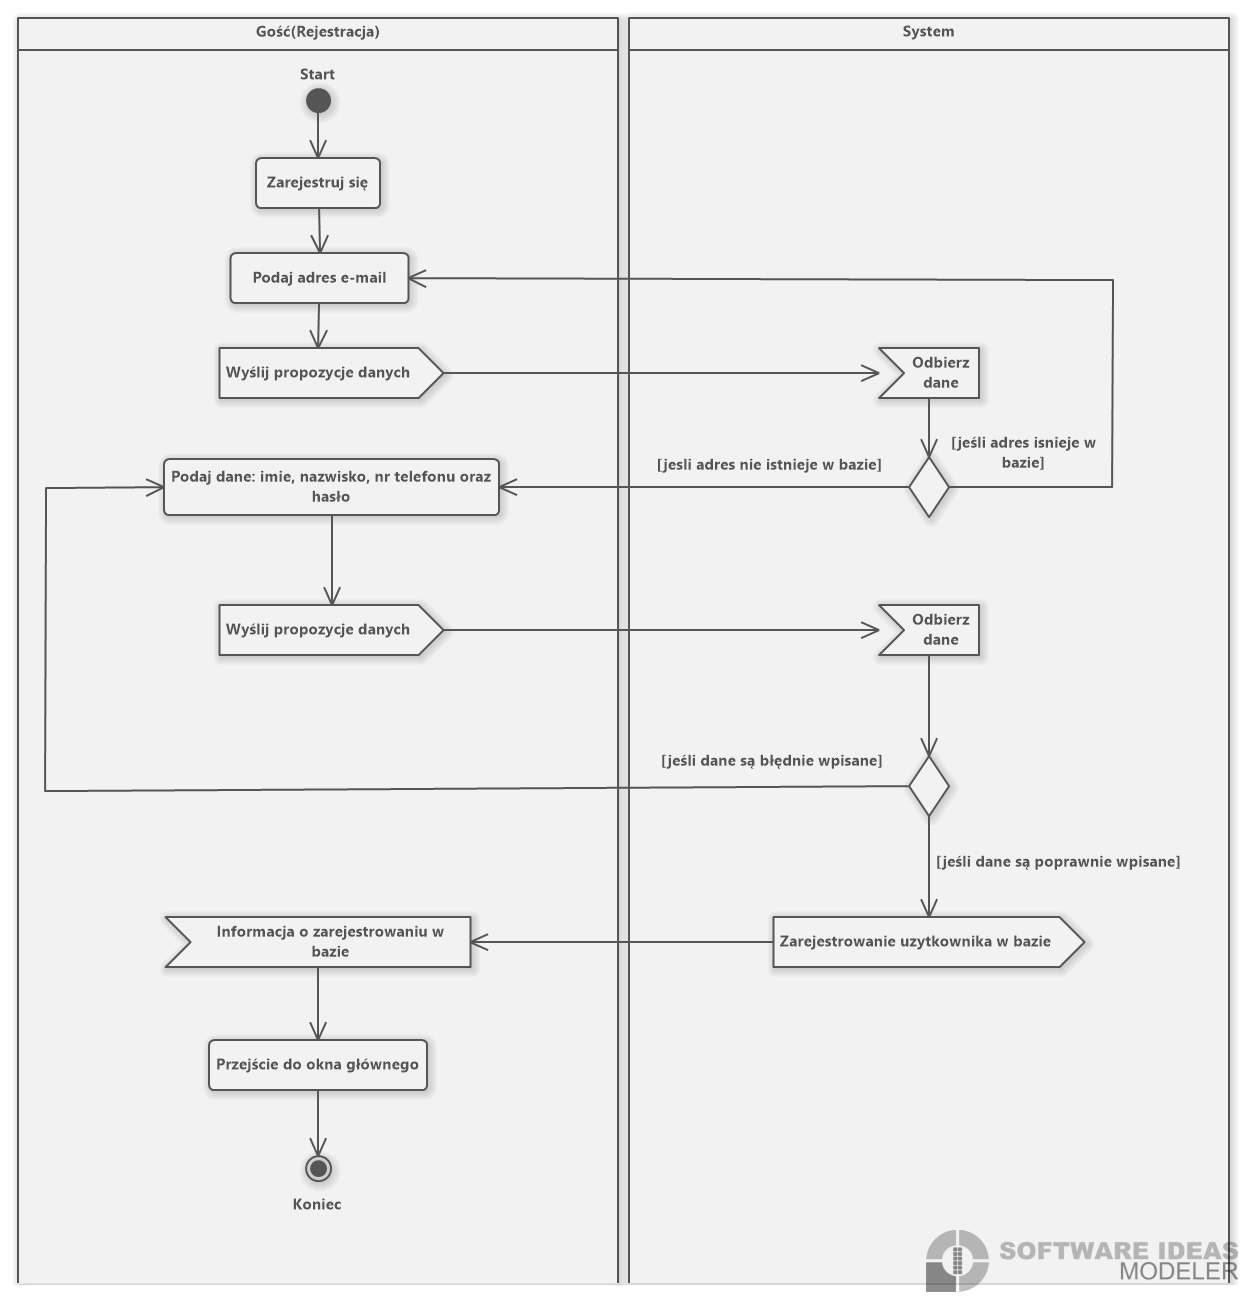
\includegraphics[scale=0.5]{acrejestracja}\\
			\caption{Rys.3 Diagram aktywności - Rejestracja}
		\end{center}
		
%--------------------------------------------------------------------------------------------------
%       DIAGRAM CZYNNOŚCI
%--------------------------------------------------------------------------------------------------
		\subsection{Diagram czynności}
		
%--------------------------------------------------------------------------------------------------
%       DIAGRAM SEKWENCJI
%--------------------------------------------------------------------------------------------------
		\subsection{Diagram sekwencji}


 
\end{document}
